\documentclass{exam}

\usepackage{units} 
\usepackage{graphicx}
\usepackage[fleqn]{amsmath}
\usepackage{cancel}
\usepackage{float}
\usepackage{mdwlist}
\usepackage{booktabs}
\usepackage{cancel}
\usepackage{polynom}
\usepackage{caption}
\usepackage{fullpage}
\usepackage{xfrac}
\usepackage{enumerate}

\newcommand{\degree}{\ensuremath{^\circ}} 
\everymath{\displaystyle}

\printanswers

% \begin{figure}[H]
%   \centering
%   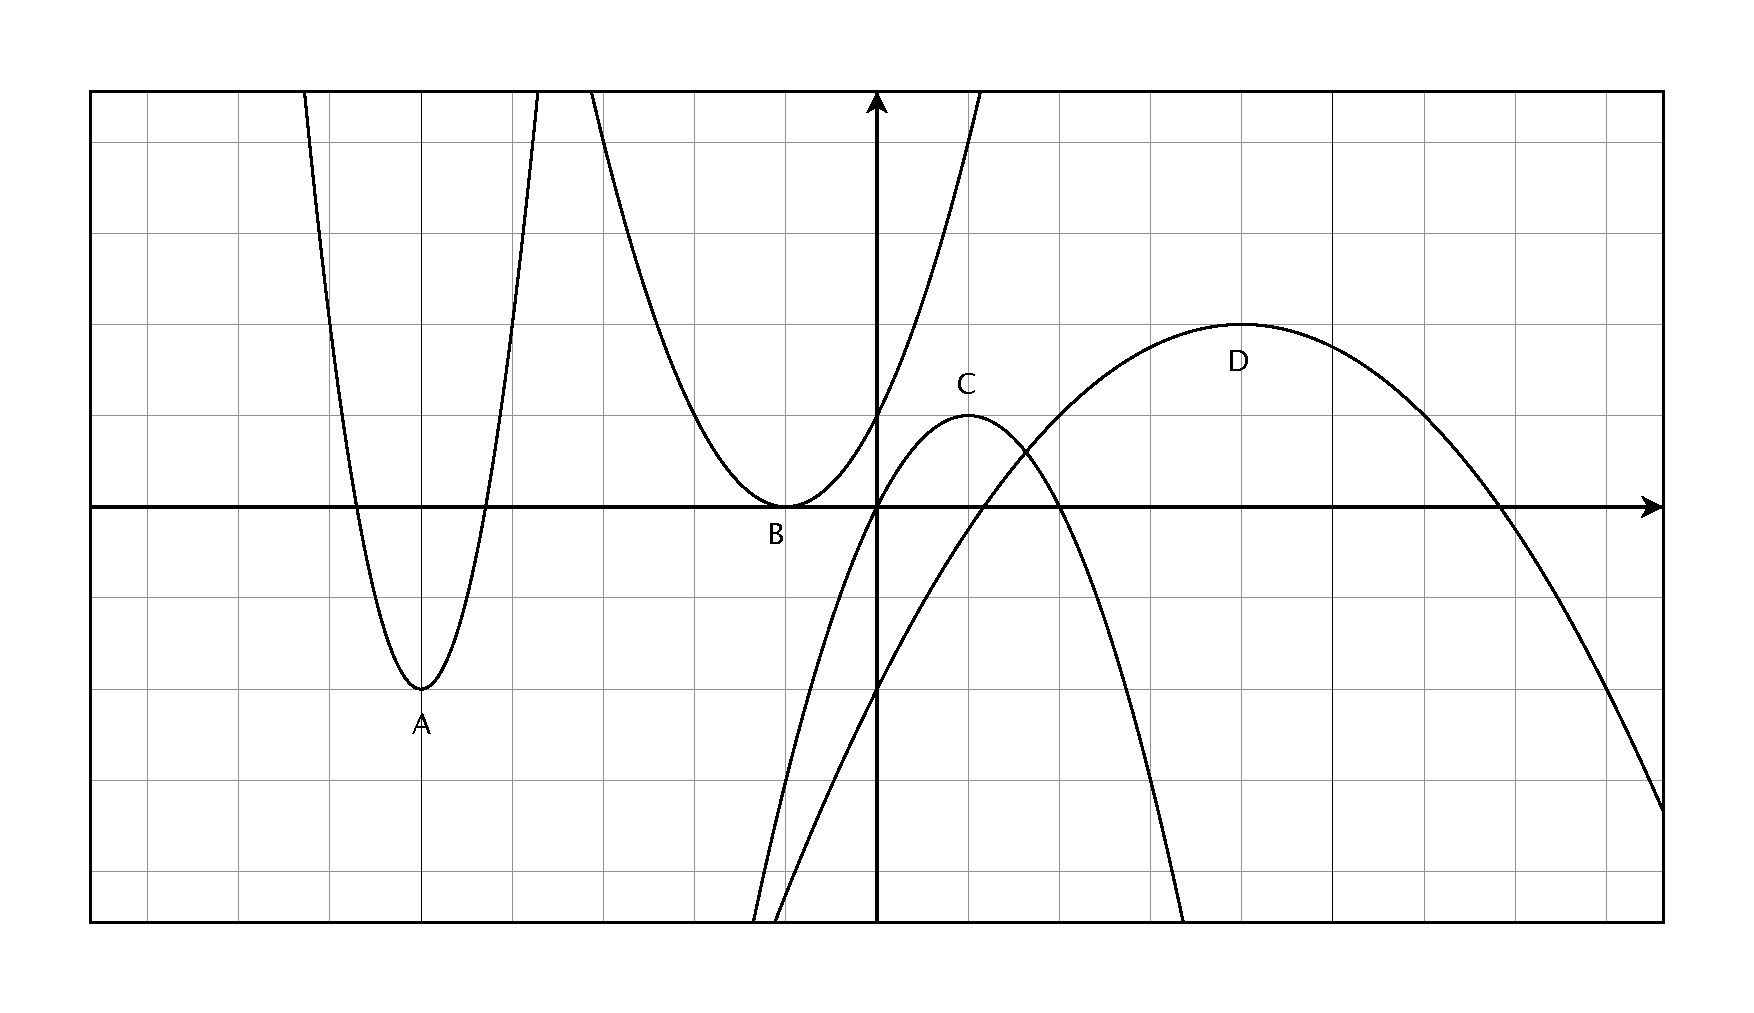
\includegraphics[scale=.3]{problem_7.eps}
%   \caption*{Problem 7}
% \end{figure}

% \begin{tabular}{cc}
% \toprule
% period & amplitude \\
% \midrule
%   $\pi$ & $2$ \\
% \bottomrule
% \end{tabular}

\title{Math 141 Notes \\ Section 4.3}

\date{June 19, 2013}

\begin{document}

  \maketitle
  \tableofcontents


  \section{Rules of Exponents Review}

  \subsection{Rules}
  \begin{align*}
    x^a \cdot x^b        &= x^{a + b} \\
    \frac{x^a}{x^b}      &= x^{a - b} \\
    \left( x^a \right)^b &= x^{ab} \\
  \end{align*}

  \section{Rules of Logarithms}

  \subsection{Rules}

  \begin{align*}
    m &= b^x \\
    x &= \log_b m \\
    \\
    n &= b^y \\
    y &= \log_b n \\
  \end{align*}

  multiplying
  \begin{align*}
    \log_b \left( mn \right) &= \log_b \left( b^x \cdot b^y \right) \\
                             &= \log_b b^{x + y} \\
                             &= x + y \\
                             &= \log_b m + \log_b n \\
  \end{align*}

  dividing
  \begin{align*}
    \log_b \left( \frac{m}{n} \right) &= \log_b \left( \frac{b^x}{b^y} \right) \\
                             &= \log_b b^{x - y} \\
                             &= x - y \\
                             &= \log_b m - \log_b n \\
  \end{align*}

  powers
  \begin{align*}
    \log_b m^z &= \log_b \left( b^x \right)^z \\
               &= \log_b b^{xz} \\
               &= xz \\
               &= z \log_b m \\
  \end{align*}

  \subsection{Examples}

  \begin{enumerate}
    \item $\log_4 \sqrt{64} = \frac{3}{5}$

    \item $\log_2 48 - \log_2 3 = \log_2 16 = 4$

    \item $\log 50 + \log 20 = \log 1000 = 3$

    \item 
      \begin{align*}
        \log_4 80 - \log_4 5 &= \log_4 \frac{80}{5} \\
                             &= \log_4 16 \\
                             &= 2 \\
      \end{align*}

    \item
      \begin{align*}
        \log_{15} 25 + \log_{15} 9 &= \log_{15} 225 \\
                                   &= 4 \\
      \end{align*}

    \item
      \begin{align*}
        \log_4 \frac{1}{32} &= \log_4 2^{-5} \\
                            &= -5 \log_4 4^{1/2} \\
                            &= - \frac{5}{2} \\
      \end{align*}

    \item
      \begin{align*}
        log_2 20 + \log_2 6 - \log_2 30 &= \log_2 \frac{20 \cdot 6}{30} \\
                                        &= \log_2 4 \\
                                        &= 2 \\
      \end{align*}

    \item 
      \begin{align*}
        \log_2 \left( 2x \right) &= \log_2 2 + \log_2 x \\
                                 &= \boxed{1 + \log_2 x} \\
      \end{align*}

    \item 
      \begin{align*}
        \log_3 \left( 5y \right) &= \log_3 5 + \log_3 y \\
                                 &= \boxed{1 + \log_3 y} \\
      \end{align*}

    \item $\log(2x)$

    \item $\log \frac{x}{2}$

    \item $\log(x^3)$

    \item $\log(x^3 y^2)$

    \item $\log \frac{x^3 \sqrt{y}}{2}$

    \item $\log 2 + \log 3$

    \item $2 \log x - \log (x - 1)$

      \item 
        \begin{align*}
          \ln \sqrt{ab} &= \ln (ab)^{1/2} \\
                        &= \frac{1}{2} \ln (ab) \\
                        &= \boxed{\frac{1}{2} (\ln a + \ln b)} \\
        \end{align*}

      \item
        \begin{align*}
          \log \sqrt{\sqrt{7}} &= \log \left( 7^{1/2} \right)^{1/2} \\
                               &= \frac{1}{2} \log 7^{1/2} \\
                               &= \frac{1}{4} \log 7 \\
        \end{align*}

      \item 
        \begin{align*}
          \ln \sqrt{3 r^2 s} &= \frac{1}{3} \ln \left( 3r^2s \right) \\
                             &= \frac{1}{3} \left( \ln 3 + \ln r^2 + \ln s \right) \\
                             &= \frac{1}{3} \left( \ln 3 + 2 \ln r + \ln s \right) \\
        \end{align*}

      \item 
        \begin{align*}
          \log \left( \frac{x^3y^4}{z^6} \right) &= \log x^3y^4 - \log z^6 \\
                                                 &= \log x^3 + \log y^4 - 6 \log z \\
                                                 &= \boxed{3 \log x + 4 \log y - 6 \log z} \\
        \end{align*}

      \item 
        \begin{align*}
          \log \left( \frac{a^2}{b^4 \sqrt{c}} \right) &= \log a^2 - \log b^4 c^{1/2} \\
                                                       &= \log a^2 - \left( \log b^4 + \log c^{1/2} \right) \\
                                                       &= \boxed{2 \log a - 4 \log b + \frac{1}{2} \log c} \\
        \end{align*}

      \item 
        \begin{align*}
          \log_2 \left( \frac{x \left( x^2 + 1 \right)}{\sqrt{x^2 - 1}} \right)
            &= \log_2 \left( x \left( x^2 + 1 \right) \right) - \frac{1}{2} \log_2 \left( x^2 - 1 \right) \\
            &= \boxed{\log_2 x + \log_2 \left( x^2 + 1 \right) - \frac{1}{2} \log_2 \left( x^2 - 1 \right)} \\
        \end{align*}

      \item 
        \begin{align*}
          \log_5 \sqrt{ \frac{x - 1}{x + 1}} &= \frac{1}{2} \log_5 \left( \frac{x - 1}{x + 1} \right) \\
                                             &= \boxed{\frac{1}{2} \left( \log_5 (x - 1) - \log_5 (x + 1) \right)} \\
        \end{align*}

  \end{enumerate}

  \section{Change of Base}

  \subsection{Rules}

  If you know logarithms in some base (base a) you can find logarithms in any other base (base b):

  \begin{align*}
    y          &= \log_b x \\
    b^y        &= x \\
    \log_a b^y &= \log_a x \\
    y \log_a b &= \log_a x \\
    y          &= \frac{\log_a x}{\log_b x} \\
    \log_b x   &= \frac{\log_a x}{\log_b x} \\
  \end{align*}

  Alternate:
  \begin{align*}
    y        &= \log_b x \\
    b^y      &= x \\
    \\
    b        &= a^{\log_a b} \\
    b^y      &= a^{y \log_a b} \\
    x        &= a^{y \log_a b} \\
    \log_a x &= y \log_a b \\
    y        &= \frac{\log_a x}{\log_a b} \\
    \log_b x &= \frac{\log_a x}{\log_a b} \\
  \end{align*}

  \subsection{Examples}

  \begin{enumerate}
    \item $\log_5 17 = \frac{\ln 17}{\ln 5}$ 
    \item etc.
  \end{enumerate}
\end{document}
